% Anonymous TMLR submission source. Compile with pdfLaTeX on Overleaf.
% Upload this file and the figures/ directory; no separate bibliography is needed.
% The unmodified official TMLR style is embedded below to keep this delivery
% self-contained. Source: JmlrOrg/tmlr-style-file, revision
% 7bf90efe3a0debbba703c05c43f3ff7e4d4a2992 (Apache-2.0).
% Its license is reproduced after end-of-document for standalone redistribution.
% Do not select accepted/preprint mode for double-blind submission.
\begin{filecontents*}{tmlr.sty}
%%%% TMLR Macros (LaTex)
%%%% Adapted by Hugo Larochelle and Fabian Pedregosa from the 
%%%% ICLR stylefile Macros and borrowing from the JMLR Macros
%%%% Style File

%%%% Last edited, January 2021 by Chris J. Maddison
%%%%      Change font choice

% Change the overall width of the page.  If these parameters are
%       changed, they will require corresponding changes in the
%       maketitle section.
%
\usepackage{eso-pic} % used by \AddToShipoutPicture
\RequirePackage{fancyhdr}
\RequirePackage{natbib}

\usepackage[T1]{fontenc}
\usepackage{lmodern}

% modification to natbib citations
\setcitestyle{authoryear,round,citesep={;},aysep={,},yysep={;}}

\renewcommand{\topfraction}{0.95}   % let figure take up nearly whole page
\renewcommand{\textfraction}{0.05}  % let figure take up nearly whole page


%%%%%%%% Options
\newif\if@accepted\@acceptedfalse
\DeclareOption{accepted}{%
    \@acceptedtrue
}
% declare preprint option, which creates a preprint version ready for
% upload to, e.g., arXiv
\newif\if@preprint\@preprintfalse
\DeclareOption{preprint}{
  \@preprinttrue
  \@acceptedtrue
}

\DeclareOption*{\PackageWarning{tmlr}{Unknown ‘\CurrentOption’}}
\ProcessOptions\relax

% Specify the dimensions of each page

\setlength{\paperheight}{11in}
\setlength{\paperwidth}{8.5in}


\oddsidemargin 0in    %   Note \oddsidemargin = \evensidemargin
\evensidemargin 0in
\marginparwidth 0.07 true in
%\marginparwidth 0.75 true in
%\topmargin 0 true pt           % Nominal distance from top of page to top of
%\topmargin 0.125in
\topmargin -0.625in
\addtolength{\headsep}{0.25in}
\textheight 9.0 true in       % Height of text (including footnotes & figures)
\textwidth 6.5 true in        % Width of text line.
\widowpenalty=10000
\clubpenalty=10000


% \thispagestyle{empty}        \pagestyle{empty}
\flushbottom \sloppy

% We're never going to need a table of contents, so just flush it to
% save space --- suggested by drstrip@sandia-2
\def\addcontentsline#1#2#3{}

% Title stuff, taken from deproc.
\def\maketitle{\par
\begingroup
   \def\thefootnote{\fnsymbol{footnote}}
   \def\@makefnmark{\hbox to 0pt{$^{\@thefnmark}$\hss}} % for perfect author
                                                        % name centering
%   The footnote-mark was overlapping the footnote-text,
%   added the following to fix this problem               (MK)
   \long\def\@makefntext##1{\parindent 1em\noindent
                            \hbox to1.8em{\hss $\m@th ^{\@thefnmark}$}##1}
   \@maketitle \@thanks
\endgroup
\setcounter{footnote}{0}
\let\maketitle\relax \let\@maketitle\relax
\gdef\@thanks{}\gdef\@author{}\gdef\@title{}\let\thanks\relax}

\newlength\aftertitskip     \newlength\beforetitskip
\newlength\interauthorskip  \newlength\aftermaketitskip

%% Changeable parameters.
\setlength\aftertitskip{0.3in plus 0.2in minus 0.2in}
\setlength\beforetitskip{0.05in plus 0.08in minus 0.08in}
\setlength\interauthorskip{0.08in plus 0.1in minus 0.1in}
\setlength\aftermaketitskip{0.3in plus 0.1in minus 0.1in}

\def\@startauthor{\noindent \normalsize\bf}
\def\@endauthor{}

\def\addr{\small\it}%
\def\email{\hfill\small\it}%
\def\name{\normalsize\bf}%
\def\name{\normalsize\bf}%
\def\AND{\@endauthor\rm\hss \vskip \interauthorskip \@startauthor}

% The toptitlebar has been raised to top-justify the first page

\usepackage{fancyhdr}
\pagestyle{fancy}
\fancyhead{}

\if@accepted
    \if@preprint
        \lhead{}
    \else
        \lhead{Published in Transactions on Machine Learning Research (\month/\year)}
    \fi
\else
       \lhead{Under review as submission to TMLR}
\fi

% Title (includes both anonymized and non-anonymized versions)
\def\@maketitle{\vbox{\hsize\textwidth
%\linewidth\hsize \vskip 0.1in \toptitlebar \centering
{\LARGE\bf\sffamily \@title\par}\vskip \aftertitskip
%\bottomtitlebar % \vskip 0.1in %  minus
\if@accepted
    \if@preprint
        \@startauthor \@author \@endauthor
    \else
        \@startauthor \@author \\ \\ {\bf Reviewed on OpenReview:} \openreview \@endauthor
    \fi
\else
    \@startauthor Anonymous authors\\Paper under double-blind review \@endauthor
\fi
\vskip 0.3in minus 0.1in}}

\renewenvironment{abstract}{\vskip.075in\centerline{\large\bf\sffamily
Abstract}\vspace{0.5ex}\begin{quote}}{\par\end{quote}\vskip 1ex}

% sections with less space
\def\section{\@startsection {section}{1}{\z@}{-2.0ex plus
    -0.5ex minus -.2ex}{1.5ex plus 0.3ex
minus0.2ex}{\large\bf\raggedright\sffamily}}

\def\subsection{\@startsection{subsection}{2}{\z@}{-1.8ex plus
-0.5ex minus -.2ex}{0.8ex plus .2ex}{\normalsize\bf\raggedright\sffamily}}
\def\subsubsection{\@startsection{subsubsection}{3}{\z@}{-1.5ex
plus      -0.5ex minus -.2ex}{0.5ex plus
.2ex}{\normalsize\bf\raggedright\sffamily}}
\def\paragraph{\@startsection{paragraph}{4}{\z@}{1.5ex plus
0.5ex minus .2ex}{-1em}{\normalsize\bf}}
\def\subparagraph{\@startsection{subparagraph}{5}{\z@}{1.5ex plus
  0.5ex minus .2ex}{-1em}{\normalsize\bf}}
\def\subsubsubsection{\vskip
5pt{\noindent\normalsize\rm\raggedright\sffamily}}


% Footnotes
\footnotesep 6.65pt %
\skip\footins 9pt plus 4pt minus 2pt
\def\footnoterule{\kern-3pt \hrule width 12pc \kern 2.6pt }
\setcounter{footnote}{0}

% Lists and paragraphs
\parindent 0pt
\topsep 4pt plus 1pt minus 2pt
\partopsep 1pt plus 0.5pt minus 0.5pt
\itemsep 2pt plus 1pt minus 0.5pt
\parsep 2pt plus 1pt minus 0.5pt
\parskip .5pc


%\leftmargin2em
\leftmargin3pc
\leftmargini\leftmargin \leftmarginii 2em
\leftmarginiii 1.5em \leftmarginiv 1.0em \leftmarginv .5em

%\labelsep \labelsep 5pt

\def\@listi{\leftmargin\leftmargini}
\def\@listii{\leftmargin\leftmarginii
   \labelwidth\leftmarginii\advance\labelwidth-\labelsep
   \topsep 2pt plus 1pt minus 0.5pt
   \parsep 1pt plus 0.5pt minus 0.5pt
   \itemsep \parsep}
\def\@listiii{\leftmargin\leftmarginiii
    \labelwidth\leftmarginiii\advance\labelwidth-\labelsep
    \topsep 1pt plus 0.5pt minus 0.5pt
    \parsep \z@ \partopsep 0.5pt plus 0pt minus 0.5pt
    \itemsep \topsep}
\def\@listiv{\leftmargin\leftmarginiv
     \labelwidth\leftmarginiv\advance\labelwidth-\labelsep}
\def\@listv{\leftmargin\leftmarginv
     \labelwidth\leftmarginv\advance\labelwidth-\labelsep}
\def\@listvi{\leftmargin\leftmarginvi
     \labelwidth\leftmarginvi\advance\labelwidth-\labelsep}

\abovedisplayskip 7pt plus2pt minus5pt%
\belowdisplayskip \abovedisplayskip
\abovedisplayshortskip  0pt plus3pt%
\belowdisplayshortskip  4pt plus3pt minus3pt%


\def\toptitlebar{\hrule height4pt\vskip .25in\vskip-\parskip}

\def\bottomtitlebar{\vskip .29in\vskip-\parskip\hrule height1pt\vskip
.09in} %
\end{filecontents*}

\documentclass[10pt]{article}
\usepackage{tmlr}
\usepackage{amsmath,amssymb,booktabs,graphicx,array,tabularx}
\usepackage{etoolbox}
\usepackage{xurl}
\usepackage[hidelinks]{hyperref}
\hypersetup{pdftitle={Subject-Independent Evaluation of Mamba for Parkinson's Disease Detection from Gait Signals},pdfauthor={},pdfsubject={Anonymous research manuscript},pdfkeywords={gait classification, selective state spaces, participant-disjoint evaluation}}
\graphicspath{{figures/}}
\newcommand{\doi}[1]{\href{https://doi.org/#1}{doi:\nolinkurl{#1}}.}

% REQUIRED BEFORE SUBMISSION: put the actual, tested anonymous mirror URL here.
% Leave empty until the mirror exists; never substitute an identifying GitHub URL.
\newcommand{\AnonymousCodeURL}{}
\newcommand{\AnonymousCodeLink}{%
  \ifdefempty{\AnonymousCodeURL}
    {\textbf{[Anonymous repository URL to be inserted before submission]}}%
    {\expandafter\url\expandafter{\AnonymousCodeURL}}}

\title{Subject-Independent Evaluation of Mamba for Parkinson's Disease Detection from Gait Signals}
\author{\name Anonymous authors}

\begin{document}
\maketitle

\begin{abstract}
Gait-based Parkinson's disease classification is often evaluated using many windows derived from relatively few participants. Separating windows or recordings does not necessarily separate people, making the evaluation unit central to the interpretation of reported performance. We examine this problem through a compact Mamba classifier and an implementation audit of two published gait-learning systems. The documented classifier uses two selective state-space blocks of width 128, with approximately 0.275 million parameters. Its existing validation report records 88.61\% accuracy and 88.52\% macro-F1; preserved recurrent reports record 87.18\% and 84.36\% accuracy for LSTM and GRU, respectively. The original Mamba loss plot is smoother than the corresponding LSTM plot, although different optimization settings preclude attributing the difference solely to architecture. Independently, a filename-level audit shows that the two released implementations construct folds from recording boundaries rather than participant groups. A deterministic control-branch replay produces participant overlap without training either model. We distinguish this reproducible implementation finding from the exploratory model results: the latter use a single development split, have unequal evaluated sample counts, and retain unresolved run-provenance discrepancies. The study motivates participant-disjoint evaluation and compact selective state-space baselines, without claiming state-of-the-art performance, universal stability, or clinical validity.
\end{abstract}

\section{Introduction}
\label{sec:intro}
Vertical ground reaction force (VGRF) recordings provide a multichannel description of foot loading during walking. The public PhysioNet Gait in Parkinson's Disease database has consequently supported a wide range of computational approaches, from local pattern descriptors to convolutional, recurrent, and attention-based networks \citep{hausdorff2008,ertugrul2016,zhao2018,elmaachi2020,nguyen2022,naimi2024}. The practical diagnostic question is whether a model can distinguish disease status for a previously unseen participant. A high score on additional recordings of people represented during training answers a different question.

This distinction is easy to obscure in gait pipelines. Each participant may contribute several recordings, and each recording may yield many windows. Splitting at either of the latter levels can leave participant-specific characteristics shared across development and evaluation sets. This is a form of identity confounding, not a phenomenon specific to any neural architecture \citep{saeb2017,chaibub2019}. In particular, assigning every window from one file to the same fold is insufficient if another file from the same participant is assigned elsewhere. Similarly, aggregating window predictions into a recording-level decision does not repair participant overlap.

We study a compact selective state-space classifier as an alternative to more elaborate gait models. Mamba combines local convolution with input-dependent state-space updates and an efficient selective scan \citep{gu2024}. This makes it a plausible backbone for multichannel gait windows without introducing multiple sensor-specific attention branches. Our emphasis is not a new block or a new accuracy record. It is the relationship between evaluation design, the interpretation of existing results, and the behavior of a comparatively simple model.

The paper makes three bounded contributions. First, it formalizes the participant-disjoint requirement for this dataset and documents a reproducible recording-versus-participant mismatch in two public implementations. Second, it presents existing binary-classification reports and original learning curves for a two-block Mamba system and recurrent comparators. Third, it separates checkpoint-supported architecture facts, documented experimental settings, and unresolved provenance, providing an explicit account of what the evidence can and cannot establish. Cross-validation, controlled split ablations, and hybrid local-feature models are future work rather than unperformed experiments presented as results.

\section{Related work}
\label{sec:related}
\paragraph{Gait representations and neural classifiers.}
\citet{ertugrul2016} proposed shifted one-dimensional local binary patterns (1D-LBP) for gait classification. The 88.9\% MLP result is reproduced as a literature entry by \citet{elmaachi2020}; we have not independently verified participant grouping in the original LBP implementation. \citet{zhao2018} developed a hybrid spatio-temporal model. \citet{elmaachi2020} introduced parallel one-dimensional convolutional branches and reported 98.7\% final walk-level binary accuracy. Their reimplementation of the earlier hybrid model obtained 90.3\%, compared with the earlier reported 98.6\%; they discuss different evaluation procedures, not a controlled experiment isolating leakage. Transformers were subsequently studied for one-dimensional gait signals by \citet{nguyen2022}. The convolutional Transformer of \citet{naimi2024} reports 87.89\% for a four-class healthy/Hoehn--Yahr task. That number is not a binary-detection comparator.

The more recent SincPD study explicitly distinguishes segment-level headline performance from stricter subject-wise evaluation \citep{salimibadr2026}. We therefore do not claim that subject-independent evaluation is absent from the literature, or that our approach is the only one to use it. Our implementation-level conclusions concern the two pinned releases analyzed in Section~\ref{sec:audit}, not every convolutional or Transformer study.

\paragraph{Evaluation with repeated measurements.}
\citet{saeb2017} argue that validation should approximate the intended clinical use-case. \citet{chaibub2019} show how subject characteristics can confound diagnostic evaluation and develop participant-label permutation controls. These results explain why familiar-participant and unseen-participant evaluation should not be pooled into one leaderboard. They do not imply that all disease-related information disappears in a recording-wise split, nor that an observed score alone identifies its underlying mechanism.

\paragraph{Selective state spaces.}
LSTM and GRU model sequential dependencies through gated recurrent updates \citep{hochreiter1997,cho2014}. Mamba provides a different input-selective recurrence with hardware-aware parallel scanning \citep{gu2024}. Its sequence-length scaling motivates this application, but does not guarantee faster classification on a particular GPU or stronger representations than every recurrent model. We report architecture size, not an unmeasured runtime advantage.

\section{Dataset and the unit of independence}
\label{sec:data}
PhysioNet describes recordings from 93 people with Parkinson's disease and 73 controls, acquired at 100\,Hz using eight force sensors beneath each foot and two aggregate-force signals \citep{hausdorff2008}. The records originate from three contributing studies, including usual walking, dual-task walking, and rhythmic auditory stimulation \citep{frenkel2005,yogev2005,hausdorff2007}. Participant identity must retain the study prefix, rather than only the numeric identifier.

An audit of the official version-1.0.0 checksum manifest finds 306 sensor-recording filenames, 165 distinct study-qualified participant identifiers, and 54 identifiers with more than one recording. These are counts of the accessible filename inventory, not a correction of the dataset's advertised 166-person cohort. The discrepancy means that an experiment should report its actual inclusion manifest rather than infer sample size from the database description. No raw signal download is required for this filename audit.

Let $x_{s,r,w}$ denote window $w$ from recording $r$ of participant $s$, and let $y_s$ be the binary disease label. With development set $\mathcal D_{\mathrm{tr}}$ and evaluation set $\mathcal D_{\mathrm{ev}}$, unseen-participant evaluation requires
\begin{equation}
  \{s:(x_{s,r,w},y_s)\in\mathcal D_{\mathrm{tr}}\}
  \;\cap\;
  \{s:(x_{s,r,w},y_s)\in\mathcal D_{\mathrm{ev}}\}
  =\varnothing .
  \label{eq:independence}
\end{equation}
For example, the recordings \texttt{GaPt07\_01} and \texttt{GaPt07\_02} belong to the same study-qualified participant. Keeping their windows separate by file does not enforce Equation~\ref{eq:independence}. Window-level scoring, recording-level aggregation, and participant-level scoring are also different estimands even when the split itself is participant-disjoint.

The preserved Mamba and principal recurrent scripts group files by the six-character participant prefix before an 80/20 stratified split with split seed 42. This is the intended independence invariant. However, the exact file manifests and generating revision for the stored model reports were not preserved. We therefore distinguish a verified grouping operation in the available source from retrospective certification of every saved prediction.

\section{An implementation audit of recording-based folds}
\label{sec:audit}
\subsection{Scope and procedure}
We inspected the official implementations accompanying \citet{elmaachi2020} and \citet{naimi2024} at fixed source revisions listed in Appendix~\ref{app:audit}. Both create lists of recording files, shuffle those lists, and append a cumulative segment-count boundary after processing each file. The arrays named in terms of patients therefore index recordings in these code paths. The subsequent fold routine partitions those boundaries without first merging files by participant identifier. The same issue is relevant to the severity code paths: retrieving a severity label by participant ID does not itself group the participant's recordings.

To demonstrate the missing invariant without reproducing network training, we independently re-express the control-branch fold arithmetic on the official filename inventory. If there are $N_c$ selected control recordings, the cumulative boundary array has $N_c+1$ entries. For ten folds the code uses width
\begin{equation}
  q=\left\lfloor (N_c+1)/10\right\rfloor,
  \qquad \mathcal V_k=F[kq:(k+1)q],
\end{equation}
where $F$ is the shuffled recording list. This filename reduction assumes each selected recording contributes at least one segment. It does not execute the patient-branch offsets, waveform preprocessing, or neural models.

The replay uses a fresh Python pseudorandom generator with seed 42 for each control subset and examines fold zero. This is an explicitly chosen audit seed, not a reconstruction of either publication's random state. The convolutional Transformer loader selects only controls with the \texttt{Ga} prefix, so its replay uses that subset. As a counterexample demonstrating the desired invariant, we also shuffle unique participant IDs and distribute complete groups over folds.

\begin{table}[t]
\caption{Metadata-only replay of the published control-branch fold construction. Overlap counts are distinct participant IDs shared by training and validation. These are not reproduced model-performance measurements.}
\label{tab:audit}
\centering
\begin{tabular}{lrrrr}
\toprule
Audited control branch & Files & Held-out files & ID overlap & Grouped overlap\\
\midrule
El Maachi et al.: all controls & 92 & 9 & 4 & 0\\
Naimi et al.: \texttt{Ga} controls & 38 & 3 & 3 & 0\\
\bottomrule
\end{tabular}
\end{table}

\subsection{Findings and their limits}
Table~\ref{tab:audit} gives the deterministic counterexamples. In the first replay, \texttt{GaCo02\_01} is held out while \texttt{GaCo02\_02} remains in training. In the second, \texttt{GaCo06\_02} is held out while \texttt{GaCo06\_01} remains in training. Participant grouping eliminates overlap in both cases. The finding is that the released recording-based construction \emph{does not enforce} Equation~\ref{eq:independence} when repeated recordings are supplied. It is stronger than inferring leakage from an unusually high accuracy, because the failure is visible in the actual partition logic.

The audit does not establish the exact inputs or folds that produced the publications' scores, measure an accuracy drop after correction, or show that their models learned only identity. A particular curated input subset could contain one recording per participant. Accordingly, the appropriate conclusion is a conditional implementation failure for repeated-recording inputs, not an allegation about intent or a blanket invalidation of the literature. Controlled retraining is needed to quantify the predictive effect.

\section{Compact Mamba classifier and documented protocol}
\label{sec:model}
\subsection{Architecture}
The documented pipeline normalizes multichannel windows, embeds each time point into a 128-dimensional representation, applies two Mamba blocks with normalization, pools over time, and predicts the two classes with a linear head (Figure~\ref{fig:architecture}). A static inspection of the saved full-model archive, without unpickling or executing it, confirms the input projection $18\rightarrow128$, two Mamba modules, three LayerNorm modules in total, and the output projection $128\rightarrow2$. Each Mamba module has state size 32, expansion factor 2, inner width 256, convolution width 32, and time-step projection rank 8. The archive contains 275,330 float32 parameter elements, consistent with these modules. Model width and state size are distinct quantities.

In simplified notation, a selective state-space recurrence updates
\begin{equation}
 h_t=\overline A_t h_{t-1}+\overline B_t u_t,
 \qquad z_t=C_t h_t+D u_t.
\end{equation}
In Mamba, input-dependent step sizes and projections provide selectivity; the continuous-time transition parameter $A$ itself is learned rather than independently regenerated from each input \citep{gu2024}. Local depthwise convolution precedes the selective scan. The model thus already combines a local operation with sequential state propagation; it is not a purely global model lacking local feature extraction.

The experimental description specifies temporal max pooling,
\begin{equation}
  v_j=\max_{1\leq t\leq T} Z_{t,j},\qquad
  \ell=W_{\mathrm{out}}v+b_{\mathrm{out}},
\end{equation}
followed by cross-entropy training. Pooling, residual wiring, and operation order are not recoverable solely from serialized module metadata. The available training script instead contains a different model definition and last-timestep selection. Figure~\ref{fig:architecture} therefore depicts the \emph{documented design}, not a claim that the historical forward pass has been reconstructed exactly. Appendix~\ref{app:provenance} records this distinction.

\begin{figure}[t]
\centering
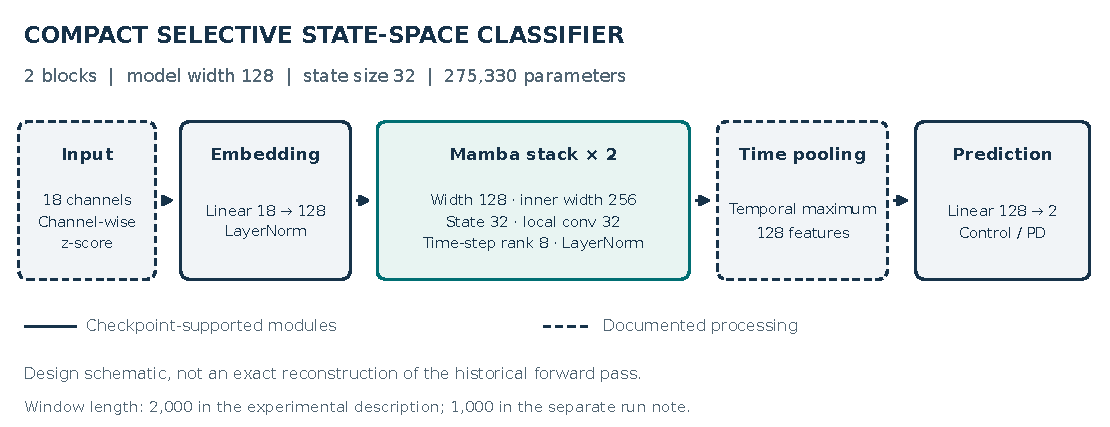
\includegraphics[width=\linewidth]{architecture.pdf}
\caption{Schematic of the documented compact classifier. Solid module boxes denote components supported by the saved model metadata; dashed processing boxes denote operations described in the experimental documentation. The schematic does not resolve the historical forward-pass discrepancy.}
\label{fig:architecture}
\end{figure}

\subsection{Preprocessing and model selection}
The experimental documentation specifies non-overlapping chunks of 2,000 timesteps (20\,s at 100\,Hz), per-channel z-score normalization, and a participant-stratified 80/20 training/validation split. A separate note for the selected Mamba run instead specifies 1,000 timesteps. The stored Mamba and recurrent reports also have different sample counts. We retain the documented settings in Table~\ref{tab:settings}, mark the window-length discrepancy, and do not assume the reports arose from identical evaluated windows.

Random hyperparameter search, validation-based learning-rate scheduling, and early stopping were used in the original workflow. The 20\% partition consequently served model development; it was not an untouched test set. Only the split seed is established by the available source. Complete initialization and training random states, the exact search budget, and repeated-seed outcomes are unavailable. A cross-validation script exists, but no completed fold-level reports are available, so no cross-validated result is claimed.

\begin{table}[t]
\caption{Settings documented for the original comparison, not a verified executable lockfile. The Mamba module dimensions are additionally supported by its saved archive. LSTM/GRU hidden sizes are per recurrent direction in the available bidirectional implementations.}
\label{tab:settings}
\centering
\begin{tabular}{lccc}
\toprule
Setting & LSTM & GRU & Mamba\\
\midrule
VGRF input channels & Selected 10 & All 18 & All 18\\
Hidden/model width & 64 & 96 & 128\\
Layers/blocks & 2 & 3 & 2\\
Batch size & 32 & 32 & 64\\
Dropout & 0.3 & 0.3 & None reported\\
Initial learning rate & $5\times10^{-3}$ & $2.5\times10^{-4}$ & $5\times10^{-5}$\\
Optimizer & Adam & Adam & Adam\\
Training objective & Binary CE & Binary CE & Weighted CE\\
Class weights & --- & --- & 1.1 / 1.0\\
Early-stopping patience & 10 & 10 & 10\\
LR-scheduler patience & 5 & 5 & 5\\
SSM state / convolution width & --- & --- & 32 / 32\\
Expansion / time-step rank & --- & --- & 2 / 8\\
Documented window length & 2,000 & 2,000 & 2,000$^{\dagger}$\\
\bottomrule
\end{tabular}

\smallskip
\begin{minipage}{0.97\linewidth}
$^{\dagger}$A separate Mamba run note states 1,000. The selected recurrent channel positions are 2, 5, 6, 8, 10, 13, 14, 16, 17, and 18 within the 18-force-channel representation. Class-weight order and unrecorded schedule details cannot be independently recovered from weights alone.
\end{minipage}
\end{table}

\section{Existing results and learning dynamics}
\label{sec:results}
\subsection{Binary classification}
Table~\ref{tab:results} transcribes the saved classification reports. Mamba records 88.61\% accuracy and 88.52\% macro-F1, numerically above the selected recurrent reports. Its control recall is 96.97\%, whereas PD recall is 80.20\%. The asymmetry is important: an overall accuracy near 89\% does not imply equally strong detection of both classes.

\begin{table}[t]
\caption{Preserved binary validation reports. Support denotes scored samples, not independent participants. Unequal supports, model selection on validation, and incomplete manifests prevent a paired ranking or a statistical superiority claim. No new training was conducted for this table.}
\label{tab:results}
\centering
\begin{tabular}{lrrrrr}
\toprule
Model & Accuracy (\%) & Macro-F1 (\%) & Control recall (\%) & PD recall (\%) & Support\\
\midrule
Mamba & 88.61 & 88.52 & 96.97 & 80.20 & 790\\
LSTM & 87.18 & 87.16 & 91.75 & 82.65 & 390\\
GRU & 84.36 & 84.34 & 88.66 & 80.10 & 390\\
\bottomrule
\end{tabular}
\end{table}

The Mamba report contains 396 control and 394 PD samples; each recurrent report contains 194 control and 196 PD samples. This is compatible with different windowing or sample preparation, but it does not identify which explanation is correct. The numerical 1.43-percentage-point Mamba--LSTM difference is therefore descriptive, not an estimate of an isolated architectural effect. We do not calculate confidence intervals treating these correlated windows as independent observations. Participant-level prediction records would be required for defensible participant-level uncertainty.

We restrict the quantitative comparison to the three binary reports with preserved class-level metrics. Exploratory feature-engineering and severity variants are outside the present empirical scope. A historical recurrent script using file-level splitting is included in the artifact as an example of the evaluation risk, not as an additional performance result.

\subsection{Observed training trajectories}
Figure~\ref{fig:loss} reproduces the original saved loss plots without smoothing, resampling, or digitizing their values. The Mamba plot shows a relatively smooth descent and subsequent validation plateau. The LSTM plot exhibits more pronounced validation fluctuations and a later rise despite decreasing training loss. These observations motivate studying training behavior separately from final accuracy.

\begin{figure}[t]
\centering
\begin{minipage}[t]{0.49\linewidth}
\centering
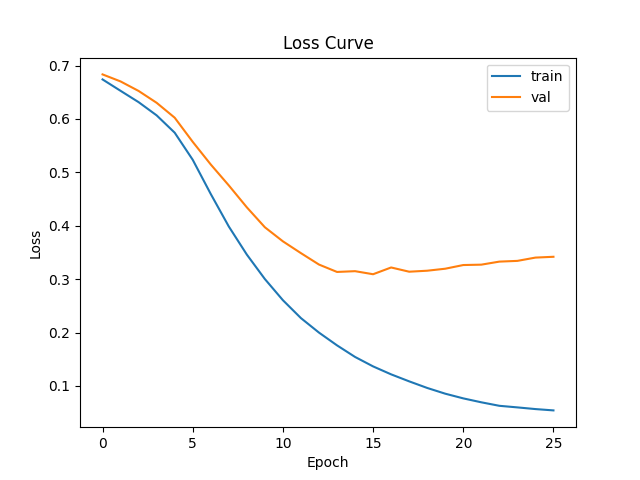
\includegraphics[width=\linewidth]{mamba_loss.png}\\
(a) Original Mamba loss plot
\end{minipage}\hfill
\begin{minipage}[t]{0.49\linewidth}
\centering
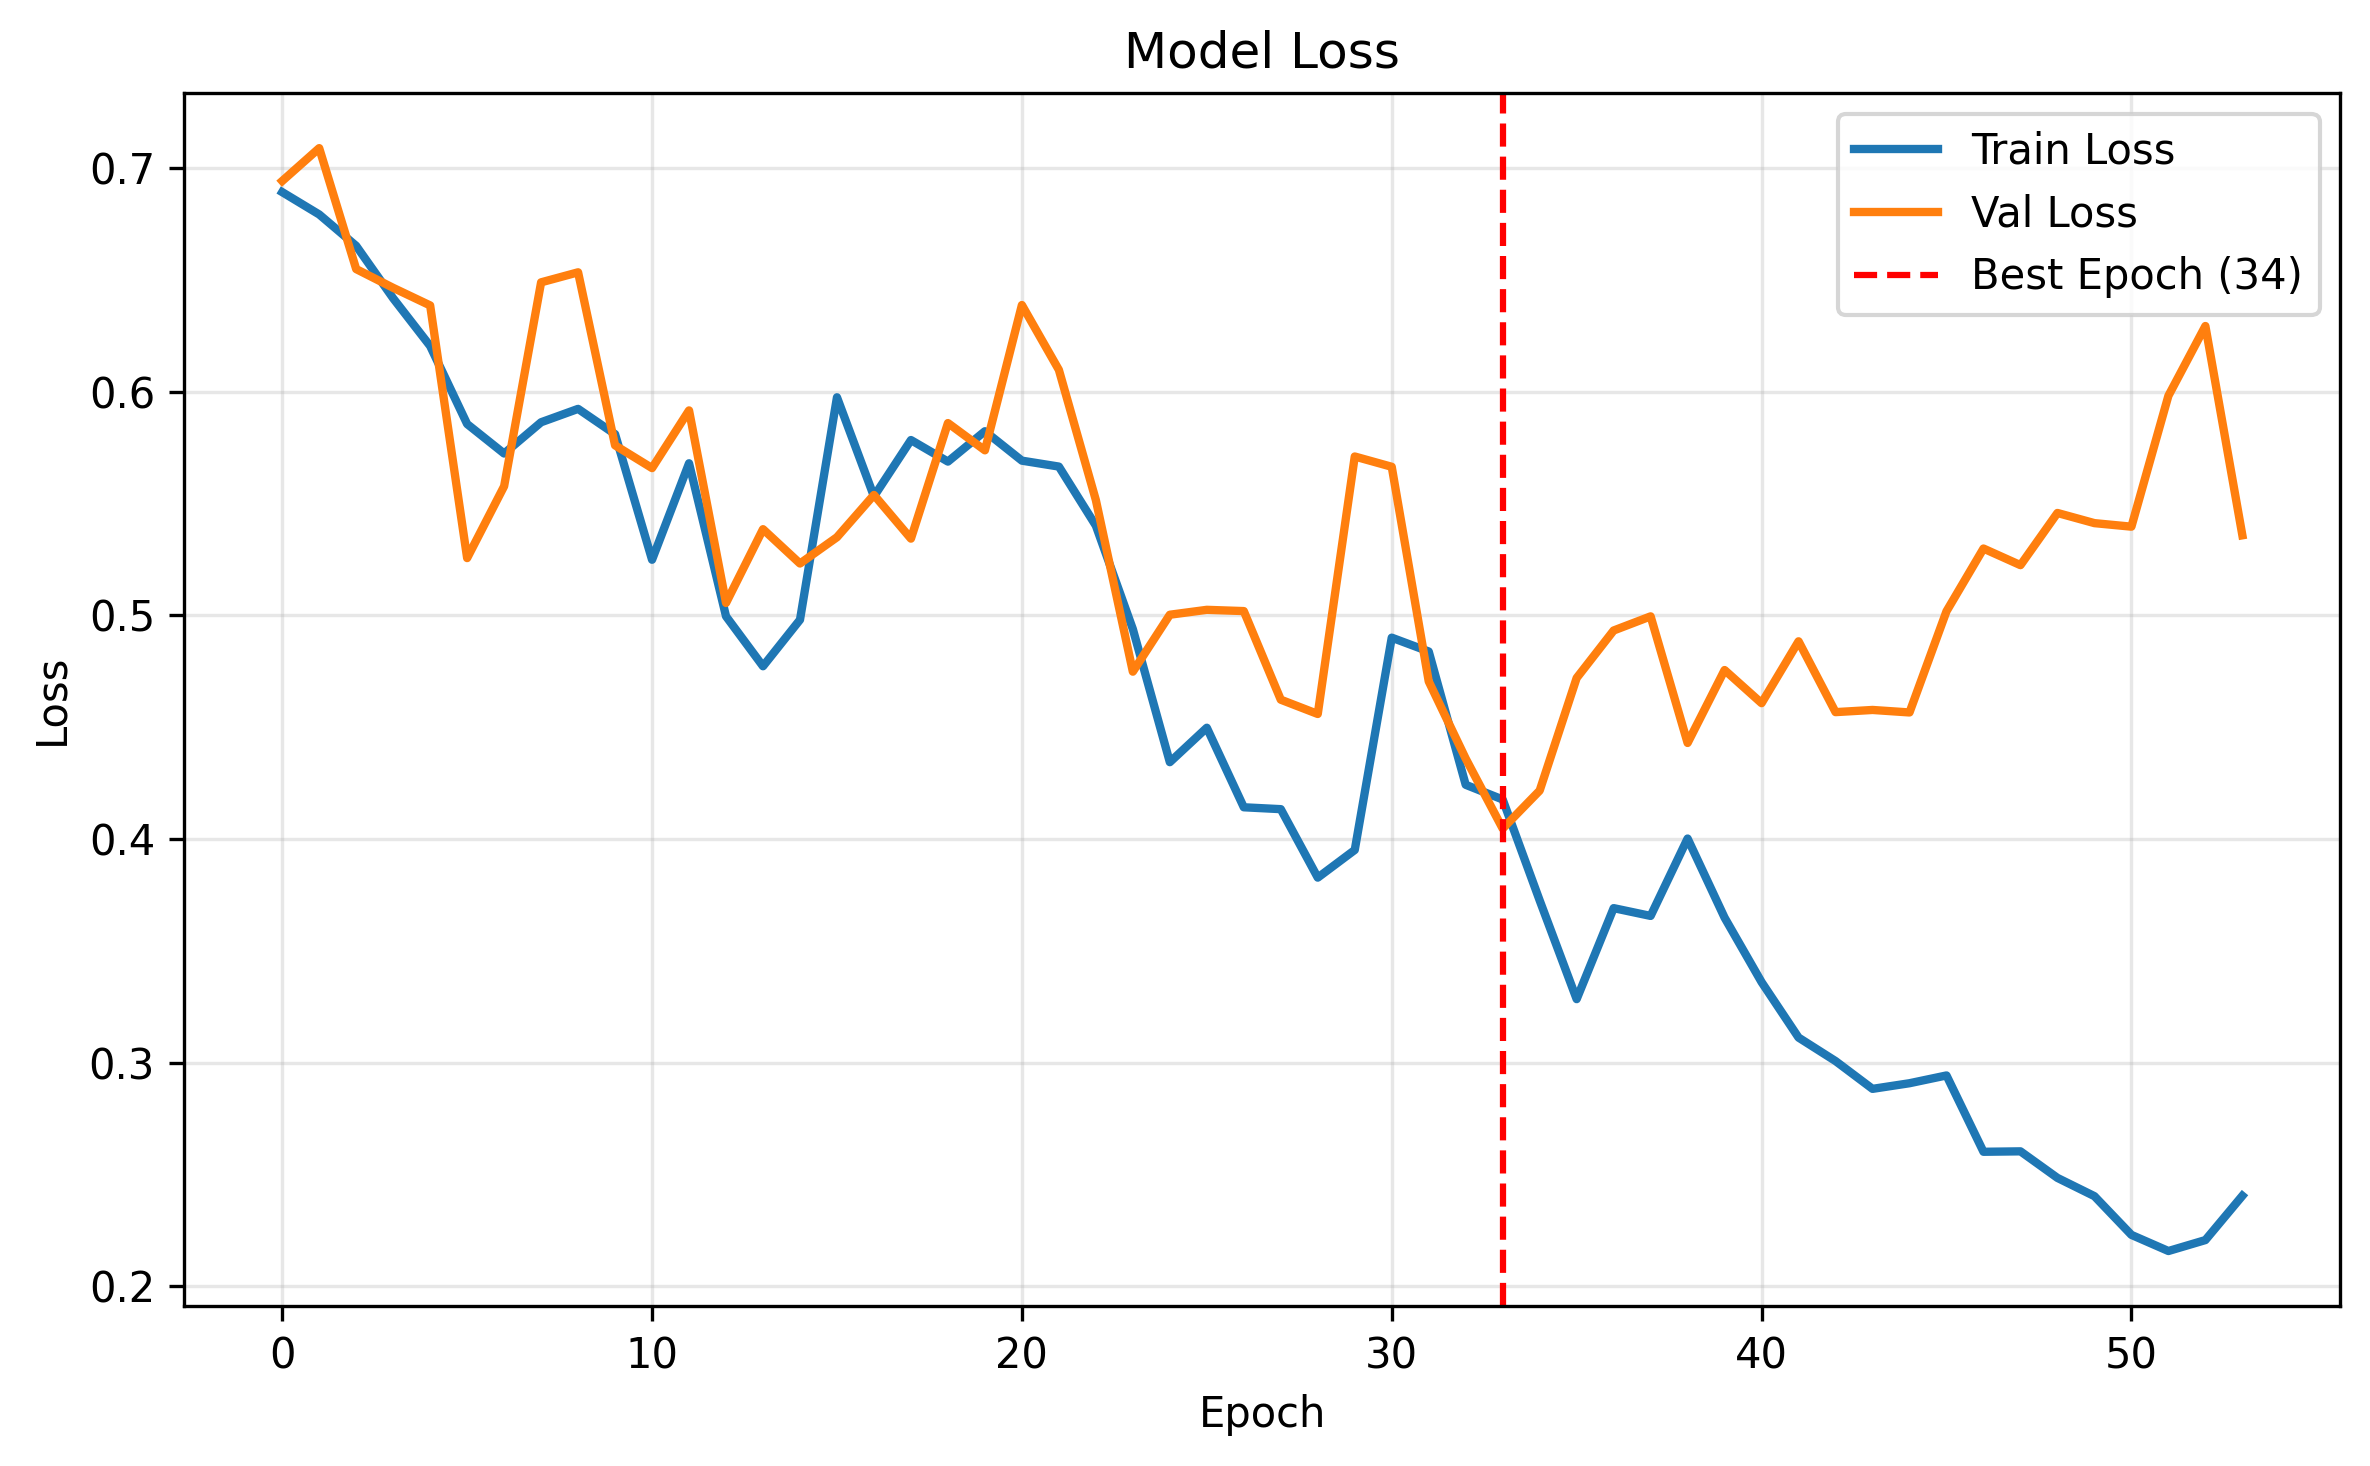
\includegraphics[width=\linewidth]{lstm_loss.png}\\
(b) Original LSTM loss plot
\end{minipage}
\caption{Original saved learning curves associated with the selected experiment folders. The plots are retained as qualitative historical evidence, not aligned repeated-run measurements. Their axes and epoch ranges are unchanged. Mamba is visibly smoother in this example, but learning rates, batch sizes, loss definitions, and evaluated sample counts differ; the plot-to-checkpoint correspondence is also incomplete. Smooth validation loss is not evidence that overfitting is absent.}
\label{fig:loss}
\end{figure}

The interpretation is deliberately narrower than ``Mamba is inherently more stable.'' Mamba's documented learning rate is 100 times smaller than LSTM's, its batch size is twice as large, and its weighted two-logit objective differs from the recurrent binary objectives. These factors can affect curve scale and smoothness. Furthermore, the Mamba validation curve eventually ceases improving while training loss continues to decrease, so a smooth curve is compatible with overfitting. Without raw epoch logs, repeated seeds, and matched tuning conditions, we cannot estimate an architecture-specific stability advantage.

\section{Discussion, limitations, and future work}
\label{sec:discussion}
\paragraph{What the current evidence establishes.}
The most directly reproducible result is the distinction between recording boundaries and participant groups in the audited code. It shows why the word ``subject'' in an implementation or evaluation description is not sufficient: the grouping key and actual membership intersection must be checked. The model artifacts provide a complementary feasibility result for a small selective state-space network, and a qualitative example of smoother learning dynamics. They do not supply a new state-of-the-art benchmark.

\paragraph{Limitations of the existing experiment.}
The validation set was used for model selection, no untouched test set or completed cross-validation result is available, and unequal report supports prevent a matched comparison. Available source and run notes disagree on some settings and do not reconstruct the selected forward pass exactly. Original split memberships and augmentation lineage are absent, so the participant-disjoint intent cannot be retroactively certified at the prediction level. These limitations apply to our own evidence as well as to comparisons with the literature. They should not be hidden by quoting more digits of accuracy. The dataset is small, mixes acquisition conditions, and does not establish transfer to new clinics, sensor systems, or populations.

\paragraph{Evaluation and stability.}
Future work should use shared outer participant folds with an inner participant-disjoint validation partition, training-only augmentation and feature selection, and explicit manifests. Window-random, recording-disjoint, and participant-disjoint variants should be compared while holding the remaining pipeline fixed. Participant-label permutation controls can test identity-related predictability \citep{chaibub2019}; they are especially straightforward for fixed binary labels and require additional care if severity changes across a participant's sessions. Repeated seeds, raw epoch logs, common evaluation objectives, and equivalent tuning budgets would turn qualitative curve observations into quantitative stability evidence. Measured latency, memory, and throughput would be needed before making efficiency claims.

\paragraph{Local features and longer temporal context.}
A CNN front end could learn multiscale cross-channel gait features or reduce temporal resolution before Mamba. Because Mamba already contains local depthwise convolution, an added stem should demonstrate a benefit beyond that built-in operation. Shifted 1D-LBP descriptors offer a complementary handcrafted alternative \citep{ertugrul2016}; computing descriptors over successive local intervals would preserve a temporal sequence for the state-space model, whereas a single recording-wide histogram would largely remove that ordering. Comparing raw-signal Mamba, CNN-only, CNN--Mamba, LBP-only, and ordered LBP--Mamba representations under shared participant folds is a natural extension. Such hybrids and preprocessing changes remain proposals, not explanations inferred from the current results.

\paragraph{Severity prediction.}
PD-only H\&Y staging, healthy-plus-stage classification, and binned UPDRS prediction are different targets. A future severity study should define the label scheme explicitly, keep every recording from a participant in one outer fold, and report class-sensitive and ordinal metrics. The present paper reports binary disease classification only; auditing severity code paths does not constitute a validated Mamba severity result.

\section{Conclusion}
Participant independence is a property of the complete data partition, not of a model architecture or a reporting label. The audited releases supply concrete examples in which recording-based folds do not guarantee that independence. Existing artifacts show that a two-block, width-128 Mamba classifier is a compact candidate for gait classification and exhibits smoother loss behavior than one recurrent comparison under its original settings. The evidence supports further participant-disjoint investigation, while leaving controlled performance, stability, and efficiency comparisons to future work.

\subsubsection*{Reproducibility and code availability}
The accompanying artifact contains the preserved aggregate reports, original loss images, anonymized historical scripts, an offline filename-audit fixture, and a nonexecuting checkpoint-metadata inspector. Historical scripts are labeled as such rather than presented as an exact reproduction of the selected run. The artifact does not redistribute participant waveforms or full serialized models. Anonymous review access: \AnonymousCodeLink.

\subsubsection*{Broader impact statement}
Improved evaluation can reduce overoptimistic claims about gait-based screening and help researchers choose simpler models on limited data. Conversely, an unvalidated classifier may miss disease or cause unnecessary concern if used as a diagnostic tool. The observed PD recall, dataset limitations, and lack of external validation preclude clinical use. This study analyzes existing de-identified public data and software; it does not recruit participants or establish prospective diagnostic benefit. No new ethics approval, regulatory clearance, or clinical endorsement is claimed.

\begin{thebibliography}{99}

\bibitem[Chaibub Neto et~al.(2019)]{chaibub2019}
Elias Chaibub Neto, Abhishek Pratap, Thanneer M. Perumal, Meghasyam Tummalacherla, Phil Snyder, Brian M. Bot, Andrew D. Trister, Stephen H. Friend, Lara Mangravite, and Larsson Omberg.
Detecting the impact of subject characteristics on machine learning-based diagnostic applications.
\emph{npj Digital Medicine}, 2:99, 2019.
\doi{10.1038/s41746-019-0178-x}

\bibitem[Cho et~al.(2014)]{cho2014}
Kyunghyun Cho, Bart van Merri\"enboer, Caglar Gulcehre, Dzmitry Bahdanau, Fethi Bougares, Holger Schwenk, and Yoshua Bengio.
Learning phrase representations using RNN encoder--decoder for statistical machine translation.
In \emph{Proceedings of EMNLP}, pp.\ 1724--1734, 2014.
\doi{10.3115/v1/D14-1179}

\bibitem[El~Maachi et~al.(2020)]{elmaachi2020}
Imanne El~Maachi, Guillaume-Alexandre Bilodeau, and Wassim Bouachir.
Deep 1D-Convnet for accurate Parkinson disease detection and severity prediction from gait.
\emph{Expert Systems with Applications}, 143:113075, 2020.
\doi{10.1016/j.eswa.2019.113075}

\bibitem[Ertu\u{g}rul et~al.(2016)]{ertugrul2016}
\"Omer Faruk Ertu\u{g}rul, Y\i lmaz Kaya, Ramazan Tekin, and Mehmet Nuri Almal\i.
Detection of Parkinson's disease by shifted one dimensional local binary patterns from gait.
\emph{Expert Systems with Applications}, 56:156--163, 2016.
\doi{10.1016/j.eswa.2016.03.018}

\bibitem[Frenkel-Toledo et~al.(2005)]{frenkel2005}
Silvi Frenkel-Toledo, Nir Giladi, Chava Peretz, Talia Herman, Leor Gruendlinger, and Jeffrey M. Hausdorff.
Treadmill walking as an external pacemaker to improve gait rhythm and stability in Parkinson's disease.
\emph{Movement Disorders}, 20(9):1109--1114, 2005.
\doi{10.1002/mds.20507}

\bibitem[Gu and Dao(2024)]{gu2024}
Albert Gu and Tri Dao.
Mamba: Linear-time sequence modeling with selective state spaces.
\emph{arXiv:2312.00752}, revised 2024.
\url{https://arxiv.org/abs/2312.00752}.

\bibitem[Hausdorff(2008)]{hausdorff2008}
Jeffrey Hausdorff.
Gait in Parkinson's Disease, version 1.0.0.
\emph{PhysioNet}, 2008.
\doi{10.13026/C24H3N}

\bibitem[Hausdorff et~al.(2007)]{hausdorff2007}
Jeffrey M. Hausdorff, J. Lowenthal, Talia Herman, Leor Gruendlinger, Chava Peretz, and Nir Giladi.
Rhythmic auditory stimulation modulates gait variability in Parkinson's disease.
\emph{European Journal of Neuroscience}, 26:2369--2375, 2007.
\doi{10.1111/j.1460-9568.2007.05810.x}

\bibitem[Hochreiter and Schmidhuber(1997)]{hochreiter1997}
Sepp Hochreiter and J\"urgen Schmidhuber.
Long short-term memory.
\emph{Neural Computation}, 9(8):1735--1780, 1997.
\doi{10.1162/neco.1997.9.8.1735}

\bibitem[Naimi et~al.(2024)]{naimi2024}
Safwen Naimi, Wassim Bouachir, and Guillaume-Alexandre Bilodeau.
1D-convolutional transformer for Parkinson disease diagnosis from gait.
\emph{Neural Computing and Applications}, 36:1947--1957, 2024. Published online in 2023.
\doi{10.1007/s00521-023-09193-6}

\bibitem[Nguyen et~al.(2022)]{nguyen2022}
Duc Minh Dimitri Nguyen, Mehdi Miah, Guillaume-Alexandre Bilodeau, and Wassim Bouachir.
Transformers for 1D signals in Parkinson's disease detection from gait.
In \emph{International Conference on Pattern Recognition}, pp.\ 5089--5095, 2022.
\doi{10.1109/ICPR56361.2022.9956330}

\bibitem[Saeb et~al.(2017)]{saeb2017}
Sohrab Saeb, Luca Lonini, Arun Jayaraman, David C. Mohr, and Konrad P. Kording.
The need to approximate the use-case in clinical machine learning.
\emph{GigaScience}, 6(5):gix019, 2017.
\doi{10.1093/gigascience/gix019}

\bibitem[Salimi-Badr et~al.(2026)]{salimibadr2026}
Armin Salimi-Badr, Mahan Veisi, and Sadra Berangi.
An explainable method based on sinc filters to diagnose Parkinson's disease severity by gait cycle analysis.
\emph{Discover Artificial Intelligence}, 6:819, 2026.
\doi{10.1007/s44163-026-01993-8}

\bibitem[Yogev et~al.(2005)]{yogev2005}
Galit Yogev, Nir Giladi, Chava Peretz, Shmuel Springer, Ely S. Simon, and Jeffrey M. Hausdorff.
Dual tasking, gait rhythmicity, and Parkinson's disease: Which aspects of gait are attention demanding?
\emph{European Journal of Neuroscience}, 22:1248--1256, 2005.
\doi{10.1111/j.1460-9568.2005.04298.x}

\bibitem[Zhao et~al.(2018)]{zhao2018}
Aite Zhao, Lin Qi, Jie Li, Junyu Dong, and Hui Yu.
A hybrid spatio-temporal model for detection and severity rating of Parkinson's disease from gait data.
\emph{Neurocomputing}, 315:1--8, 2018.
\doi{10.1016/j.neucom.2018.03.032}

\end{thebibliography}

\appendix
\section{Pinned implementation audit}
\label{app:audit}
The audited sources are the public release accompanying \citet{elmaachi2020}, revision \texttt{c5a6d5f1e2a8a53cc92f020b675fa6ad7243c372}, and the public release accompanying \citet{naimi2024}, revision \texttt{fb1ace4e6c038a87674bf8ab0610055a19737d2f}. The following are external authors' repositories, not links to the present submission's identifying repository:
\begin{itemize}
\item El Maachi et al.: \url{https://github.com/imanneelmaachi/Parkinson-disease-detection-and-severity-prediction-from-gait}. In \texttt{src/data\_utils.py}, lines 47--67 collect and shuffle files; lines 75--120 build folds; lines 195--266 load each recording and append its segment-count boundary.
\item Naimi et al.: \url{https://github.com/SafwenNaimi/1D-Convolutional-transformer-for-Parkinson-disease-diagnosis-from-gait}. In \texttt{main.py}, lines 197--212 collect and shuffle files; lines 229--276 build folds; lines 349--426 load recordings and append boundaries.
\end{itemize}
Line ranges refer to the pinned revisions. Both implementations use participant IDs when obtaining some labels, but not as the grouping unit of these fold constructors. The audit makes no inference about unpublished revisions or manually curated training subsets.

The bundled fixture is the official \url{https://physionet.org/files/gaitpdb/1.0.0/SHA256SUMS.txt} inventory, retrieved on 8 November 2026. Its SHA-256 digest is \nolinkurl{44903ce52d5428ba218a9cdfd60d5646ab6674df4926233c756ae7c3c7cd50ec}. The audit can run offline against this fixture; downloading the manifest is an explicit opt-in. The utility reports filenames, participant intersections, the audit seed, and its control-only scope. It does not fetch waveforms or execute external training code. The grouped counterexample preserves participant membership by construction; its zero overlap is not an accuracy result.

\clearpage
\section{Evidence provenance and unresolved configuration}
\label{app:provenance}
\begin{table}[h]
\caption{Evidence boundaries for the existing Mamba experiment. These qualifications are retained in the review artifact rather than silently resolved by choosing a favorable source.}
\centering
\begin{tabularx}{\linewidth}{@{}>{\raggedright\arraybackslash}p{0.23\linewidth}>{\raggedright\arraybackslash}X>{\raggedright\arraybackslash}X@{}}
\toprule
Item & Available evidence & Remaining uncertainty\\
\midrule
Model modules & Two width-128 Mamba modules; state 32; convolution 32; expansion 2; rank 8; input and output projections; three LayerNorm modules & Serialized modules do not preserve the custom forward method or exact residual/pooling sequence.\\
Window length & Experimental description: 2,000; separate selected-run note: 1,000 & No per-prediction manifest resolves which length generated the 790-sample report.\\
Convolution width & Description and model archive: 32; run note: 16 & The note is not a reliable complete configuration record.\\
Training code & Participant grouping in historical source & Its single-block call passes unsupported \texttt{n\_layers} to the bundled Mamba interface; it is not the selected checkpoint's executable definition.\\
Original plots & Preserved Mamba and LSTM raster plots & Raw epoch logs are unavailable; the Mamba plot has fewer epoch entries than checkpoint files in its folder.\\
Saved metrics & Aggregate class reports, including support & No participant-wise prediction file, paired input list, or independent final test result.\\
Severity experiments & Historical code variants & No validated Mamba severity result is supplied.\\
\bottomrule
\end{tabularx}
\end{table}

The historical scripts in the artifact preserve computational behavior, including the above limitations, while replacing identifying local input paths with configurable paths. They are evidence snapshots, not a newly validated training pipeline. The selected checkpoint is not redistributed; the inspection utility reads archive metadata and pickle opcodes without executing pickle operations or importing saved model classes. The manuscript's original plots retain their original pixel values, with nonessential image metadata removed for anonymity. The architecture schematic is newly drawn from the documented design and module evidence.

\end{document}

% Third-party license for the embedded TMLR style only.
% This notice does not license the original manuscript or experimental code.
%
%                                  Apache License
%                            Version 2.0, January 2004
%                         http://www.apache.org/licenses/
%
%    TERMS AND CONDITIONS FOR USE, REPRODUCTION, AND DISTRIBUTION
%
%    1. Definitions.
%
%       "License" shall mean the terms and conditions for use, reproduction,
%       and distribution as defined by Sections 1 through 9 of this document.
%
%       "Licensor" shall mean the copyright owner or entity authorized by
%       the copyright owner that is granting the License.
%
%       "Legal Entity" shall mean the union of the acting entity and all
%       other entities that control, are controlled by, or are under common
%       control with that entity. For the purposes of this definition,
%       "control" means (i) the power, direct or indirect, to cause the
%       direction or management of such entity, whether by contract or
%       otherwise, or (ii) ownership of fifty percent (50%) or more of the
%       outstanding shares, or (iii) beneficial ownership of such entity.
%
%       "You" (or "Your") shall mean an individual or Legal Entity
%       exercising permissions granted by this License.
%
%       "Source" form shall mean the preferred form for making modifications,
%       including but not limited to software source code, documentation
%       source, and configuration files.
%
%       "Object" form shall mean any form resulting from mechanical
%       transformation or translation of a Source form, including but
%       not limited to compiled object code, generated documentation,
%       and conversions to other media types.
%
%       "Work" shall mean the work of authorship, whether in Source or
%       Object form, made available under the License, as indicated by a
%       copyright notice that is included in or attached to the work
%       (an example is provided in the Appendix below).
%
%       "Derivative Works" shall mean any work, whether in Source or Object
%       form, that is based on (or derived from) the Work and for which the
%       editorial revisions, annotations, elaborations, or other modifications
%       represent, as a whole, an original work of authorship. For the purposes
%       of this License, Derivative Works shall not include works that remain
%       separable from, or merely link (or bind by name) to the interfaces of,
%       the Work and Derivative Works thereof.
%
%       "Contribution" shall mean any work of authorship, including
%       the original version of the Work and any modifications or additions
%       to that Work or Derivative Works thereof, that is intentionally
%       submitted to Licensor for inclusion in the Work by the copyright owner
%       or by an individual or Legal Entity authorized to submit on behalf of
%       the copyright owner. For the purposes of this definition, "submitted"
%       means any form of electronic, verbal, or written communication sent
%       to the Licensor or its representatives, including but not limited to
%       communication on electronic mailing lists, source code control systems,
%       and issue tracking systems that are managed by, or on behalf of, the
%       Licensor for the purpose of discussing and improving the Work, but
%       excluding communication that is conspicuously marked or otherwise
%       designated in writing by the copyright owner as "Not a Contribution."
%
%       "Contributor" shall mean Licensor and any individual or Legal Entity
%       on behalf of whom a Contribution has been received by Licensor and
%       subsequently incorporated within the Work.
%
%    2. Grant of Copyright License. Subject to the terms and conditions of
%       this License, each Contributor hereby grants to You a perpetual,
%       worldwide, non-exclusive, no-charge, royalty-free, irrevocable
%       copyright license to reproduce, prepare Derivative Works of,
%       publicly display, publicly perform, sublicense, and distribute the
%       Work and such Derivative Works in Source or Object form.
%
%    3. Grant of Patent License. Subject to the terms and conditions of
%       this License, each Contributor hereby grants to You a perpetual,
%       worldwide, non-exclusive, no-charge, royalty-free, irrevocable
%       (except as stated in this section) patent license to make, have made,
%       use, offer to sell, sell, import, and otherwise transfer the Work,
%       where such license applies only to those patent claims licensable
%       by such Contributor that are necessarily infringed by their
%       Contribution(s) alone or by combination of their Contribution(s)
%       with the Work to which such Contribution(s) was submitted. If You
%       institute patent litigation against any entity (including a
%       cross-claim or counterclaim in a lawsuit) alleging that the Work
%       or a Contribution incorporated within the Work constitutes direct
%       or contributory patent infringement, then any patent licenses
%       granted to You under this License for that Work shall terminate
%       as of the date such litigation is filed.
%
%    4. Redistribution. You may reproduce and distribute copies of the
%       Work or Derivative Works thereof in any medium, with or without
%       modifications, and in Source or Object form, provided that You
%       meet the following conditions:
%
%       (a) You must give any other recipients of the Work or
%           Derivative Works a copy of this License; and
%
%       (b) You must cause any modified files to carry prominent notices
%           stating that You changed the files; and
%
%       (c) You must retain, in the Source form of any Derivative Works
%           that You distribute, all copyright, patent, trademark, and
%           attribution notices from the Source form of the Work,
%           excluding those notices that do not pertain to any part of
%           the Derivative Works; and
%
%       (d) If the Work includes a "NOTICE" text file as part of its
%           distribution, then any Derivative Works that You distribute must
%           include a readable copy of the attribution notices contained
%           within such NOTICE file, excluding those notices that do not
%           pertain to any part of the Derivative Works, in at least one
%           of the following places: within a NOTICE text file distributed
%           as part of the Derivative Works; within the Source form or
%           documentation, if provided along with the Derivative Works; or,
%           within a display generated by the Derivative Works, if and
%           wherever such third-party notices normally appear. The contents
%           of the NOTICE file are for informational purposes only and
%           do not modify the License. You may add Your own attribution
%           notices within Derivative Works that You distribute, alongside
%           or as an addendum to the NOTICE text from the Work, provided
%           that such additional attribution notices cannot be construed
%           as modifying the License.
%
%       You may add Your own copyright statement to Your modifications and
%       may provide additional or different license terms and conditions
%       for use, reproduction, or distribution of Your modifications, or
%       for any such Derivative Works as a whole, provided Your use,
%       reproduction, and distribution of the Work otherwise complies with
%       the conditions stated in this License.
%
%    5. Submission of Contributions. Unless You explicitly state otherwise,
%       any Contribution intentionally submitted for inclusion in the Work
%       by You to the Licensor shall be under the terms and conditions of
%       this License, without any additional terms or conditions.
%       Notwithstanding the above, nothing herein shall supersede or modify
%       the terms of any separate license agreement you may have executed
%       with Licensor regarding such Contributions.
%
%    6. Trademarks. This License does not grant permission to use the trade
%       names, trademarks, service marks, or product names of the Licensor,
%       except as required for reasonable and customary use in describing the
%       origin of the Work and reproducing the content of the NOTICE file.
%
%    7. Disclaimer of Warranty. Unless required by applicable law or
%       agreed to in writing, Licensor provides the Work (and each
%       Contributor provides its Contributions) on an "AS IS" BASIS,
%       WITHOUT WARRANTIES OR CONDITIONS OF ANY KIND, either express or
%       implied, including, without limitation, any warranties or conditions
%       of TITLE, NON-INFRINGEMENT, MERCHANTABILITY, or FITNESS FOR A
%       PARTICULAR PURPOSE. You are solely responsible for determining the
%       appropriateness of using or redistributing the Work and assume any
%       risks associated with Your exercise of permissions under this License.
%
%    8. Limitation of Liability. In no event and under no legal theory,
%       whether in tort (including negligence), contract, or otherwise,
%       unless required by applicable law (such as deliberate and grossly
%       negligent acts) or agreed to in writing, shall any Contributor be
%       liable to You for damages, including any direct, indirect, special,
%       incidental, or consequential damages of any character arising as a
%       result of this License or out of the use or inability to use the
%       Work (including but not limited to damages for loss of goodwill,
%       work stoppage, computer failure or malfunction, or any and all
%       other commercial damages or losses), even if such Contributor
%       has been advised of the possibility of such damages.
%
%    9. Accepting Warranty or Additional Liability. While redistributing
%       the Work or Derivative Works thereof, You may choose to offer,
%       and charge a fee for, acceptance of support, warranty, indemnity,
%       or other liability obligations and/or rights consistent with this
%       License. However, in accepting such obligations, You may act only
%       on Your own behalf and on Your sole responsibility, not on behalf
%       of any other Contributor, and only if You agree to indemnify,
%       defend, and hold each Contributor harmless for any liability
%       incurred by, or claims asserted against, such Contributor by reason
%       of your accepting any such warranty or additional liability.
%
%    END OF TERMS AND CONDITIONS
%
%    APPENDIX: How to apply the Apache License to your work.
%
%       To apply the Apache License to your work, attach the following
%       boilerplate notice, with the fields enclosed by brackets "[]"
%       replaced with your own identifying information. (Don't include
%       the brackets!)  The text should be enclosed in the appropriate
%       comment syntax for the file format. We also recommend that a
%       file or class name and description of purpose be included on the
%       same "printed page" as the copyright notice for easier
%       identification within third-party archives.
%
%    Copyright [yyyy] [name of copyright owner]
%
%    Licensed under the Apache License, Version 2.0 (the "License");
%    you may not use this file except in compliance with the License.
%    You may obtain a copy of the License at
%
%        http://www.apache.org/licenses/LICENSE-2.0
%
%    Unless required by applicable law or agreed to in writing, software
%    distributed under the License is distributed on an "AS IS" BASIS,
%    WITHOUT WARRANTIES OR CONDITIONS OF ANY KIND, either express or implied.
%    See the License for the specific language governing permissions and
%    limitations under the License.
